\documentclass{article}
\usepackage[T1]{fontenc}
\usepackage[utf8]{inputenc}

\usepackage{xspace}
\usepackage{graphicx}
\usepackage{amsmath}
\usepackage{amsfonts}
\usepackage{subfig}
\usepackage{fullpage}
\usepackage{url,paralist}
\usepackage{caption}
\usepackage{slashbox}

\author{Marco Eilers\\ \url{eilers.marco@googlemail.com}}
\title{Statistical Methods for Machine Learning\\ Final Exam Assignment: Sports Analytics}
\date{}

\newcommand{\vect}[1]{\ensuremath{\boldsymbol{\mathbf{#1}}}\xspace}

%% For readability in question 1.3
\newcommand{\Target}{\vect{\mathsf{T}}}
\newcommand{\vPhi}{\vect{\Phi}}
\newcommand{\vw}{\vect{w}}
\newcommand{\Szero}{\vect{S}_0}
\newcommand{\mzero}{\vect{m}_0}
\newcommand{\target}{\vect{\mathsf{t}}}

\newcommand{\knollA}{\textsc{knollA}\xspace}
\newcommand{\knollB}{\textsc{knollB}\xspace}
\newcommand{\knollC}{\textsc{knollC}\xspace}

%% %% Uncomment these lines to get a box around all figures
%% \usepackage{float}
%% \floatstyle{boxed}
%% \restylefloat{figure}

\begin{document}
\maketitle

\section{Question 1}
I used Matlab for the implementation of all exercises, since it provides many builtin tools for statistical and matrix-related operations and is a lot faster than for example Octave or R. I used Matlab's \texttt{hist} and \texttt{bar} functions to display the histogram and normalized the data. See \texttt{q1.m} for the implementation and fig. ~\ref{fig:probdisthist} for the histogram of the probability distribution. 

\begin{figure}
  \centering
  \subfloat[\hfill]{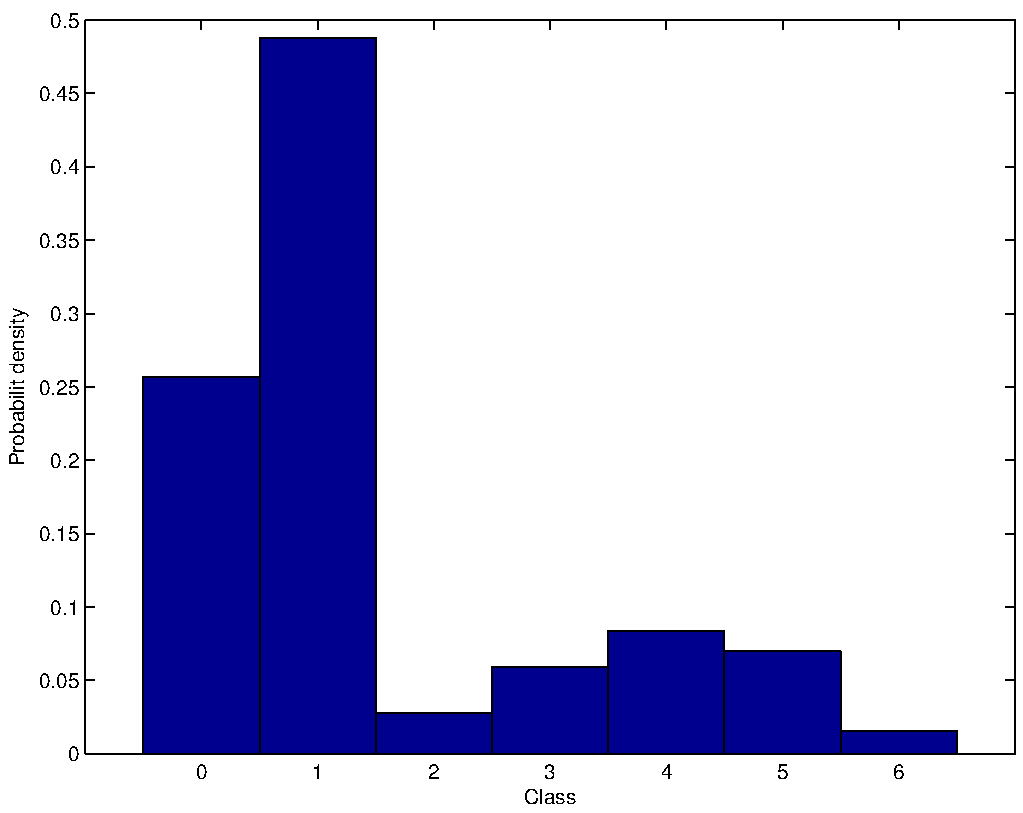
\includegraphics[width=.5\textwidth]{probdisthist.pdf}}

  \caption{Histogram showing the probability distribution of classes in the training data}
  \label{fig:probdisthist}
\end{figure}

\section{Question 2}

I implemented the Principal Component Analysis myself using Matlab's \texttt{eig} function to get eigenvectors and eigenvalues. See \texttt{q2and3.m} for the actual implementation. 15 principal components are needed to give us more than 90 percent of the total variance: they give us 90.53 percent. You can see the eigenspectrum in fig. ~\ref{fig:eigenspectrum}. It is obvious that a large amount of the total variance is indeed captured by the first few Principal Components, which is why we can expect a reduction of the data to these two components to yield relatively well-distinguishable groups.
\begin{figure}

  \subfloat[\hfill]{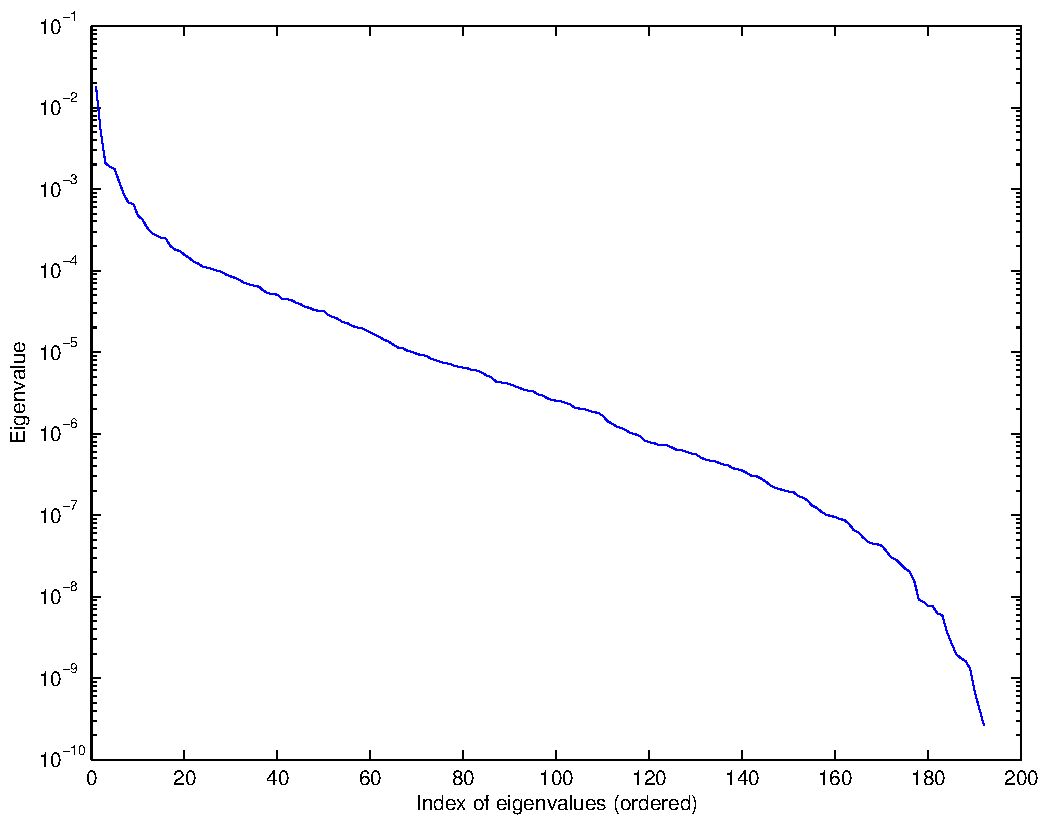
\includegraphics[width=.5\textwidth]{eigenspectrum.pdf}}
  \subfloat[\hfill]{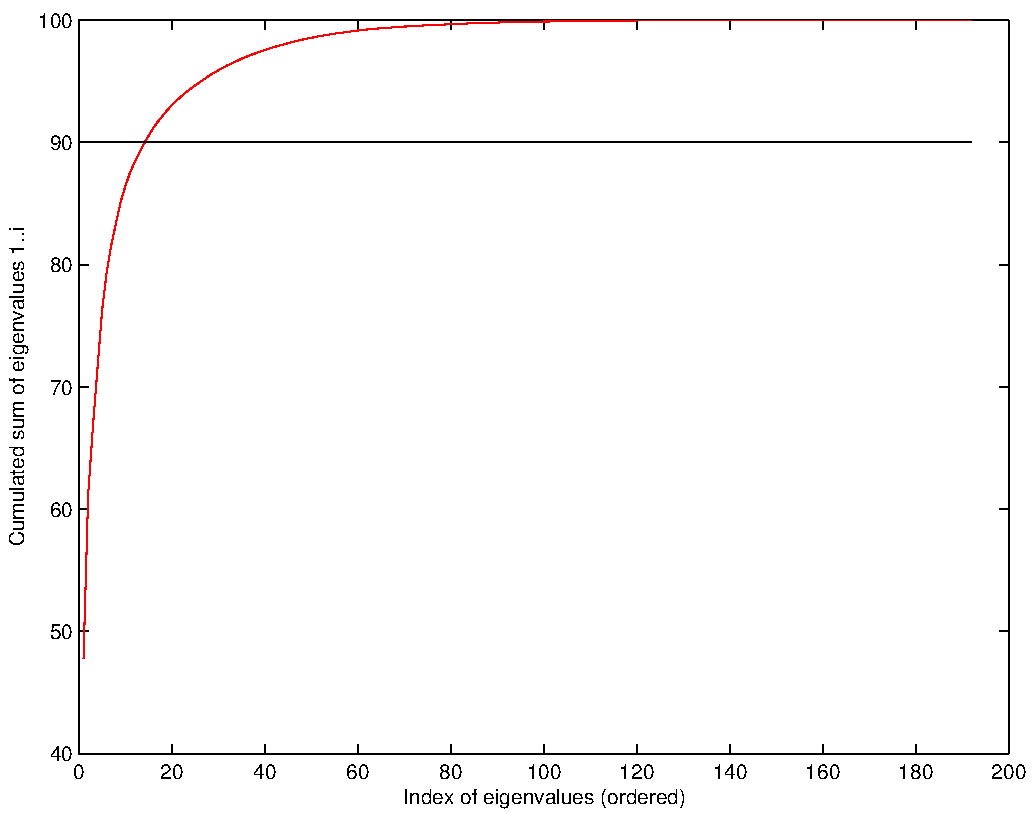
\includegraphics[width=.5\textwidth]{pcscumulatedperc.pdf}}

  \caption{Eigenspectrum and cumulated percentage of the variance for the principal components}
  \label{fig:eigenspectrum}
\end{figure}

When we project the training data to the first two principal components and visualize the result, we get fig. ~\ref{fig:pcaplot}. We can see that there are indeed some well-separated groups for classes 0, 1, 4 and 5, whereas classes 2 and 3, although somewhat separable, seem to form one block together. The error class, as can be expected, is distributed all over the place.

\begin{figure}
  \centering
  \subfloat[\hfill]{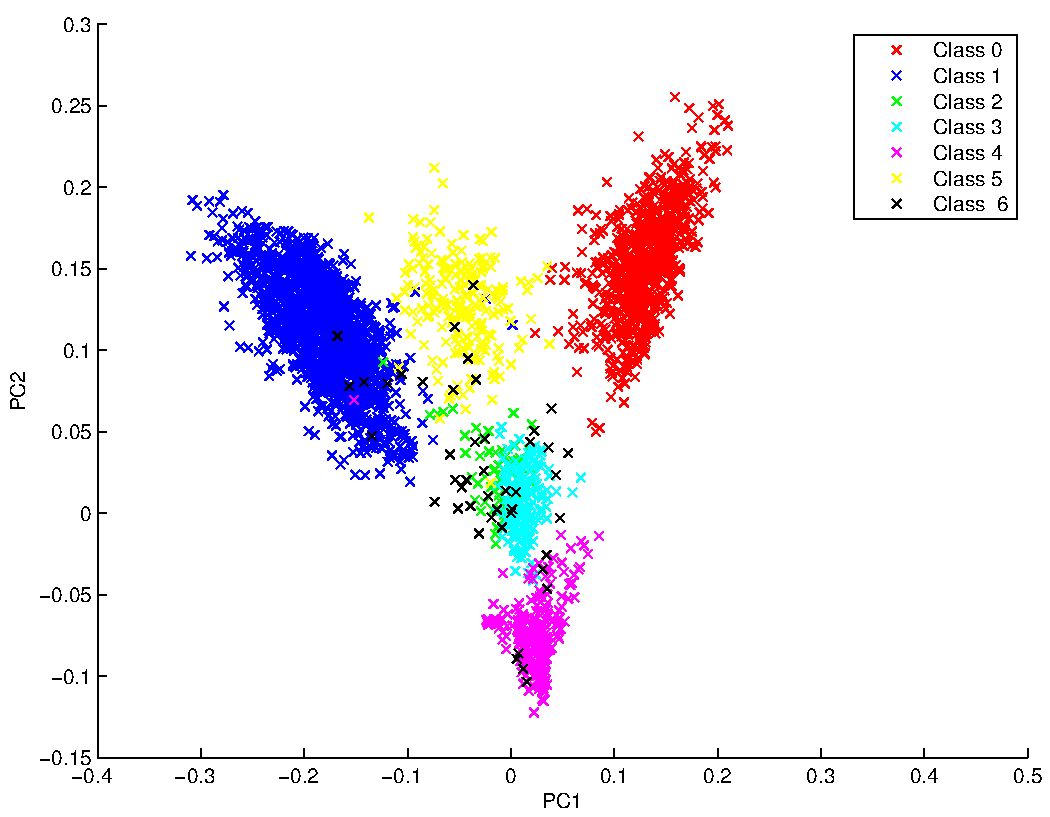
\includegraphics[width=.6\textwidth]{pcaplot.pdf}}

  \caption{Plot of the training data projected to the first two principal components}
  \label{fig:pcaplot}
\end{figure}


\section{Question 3}

I used Matlab's builtin function \texttt{kmeans} to calculate the cluster centers with the default parameters, i.e. random initial clusters and a squared euclidean distance function, and only passing the data and $k$ as arguments. See \texttt{q2and3.m} for details on the implementation. 

Projecting the cluster centers to the first two principal components and plotting the result gives results like in fig. ~\ref{fig:7meansclusters}. Since the initialization is random, different results can occur. While the algorithm always finds reasonable cluster centers for classes 0, 1 and 4, it never finds one which could reasonably be assigned to the error class, which is expected. The results for classes 2, 3 and 5 are dependent on the initialization: Often there is only one cluster center for classes 2 and 3 combined, and the centers found for class 5 often seem to miss the actual center of that cluster. This could, of course, simply be a result of the projection to the PCs, meaning that the 2D plot does not show all nuances of the data, whereas the \texttt{kmeans} works on the actual data. As a result of this, not finding the center of one class will mean that a different class (often 0 or 1) is divided into several clusters. Reducing $k$ could solve this problem, but would obviously mean that some classes will remain empty.

\begin{figure}
  \centering
  \subfloat[\hfill]{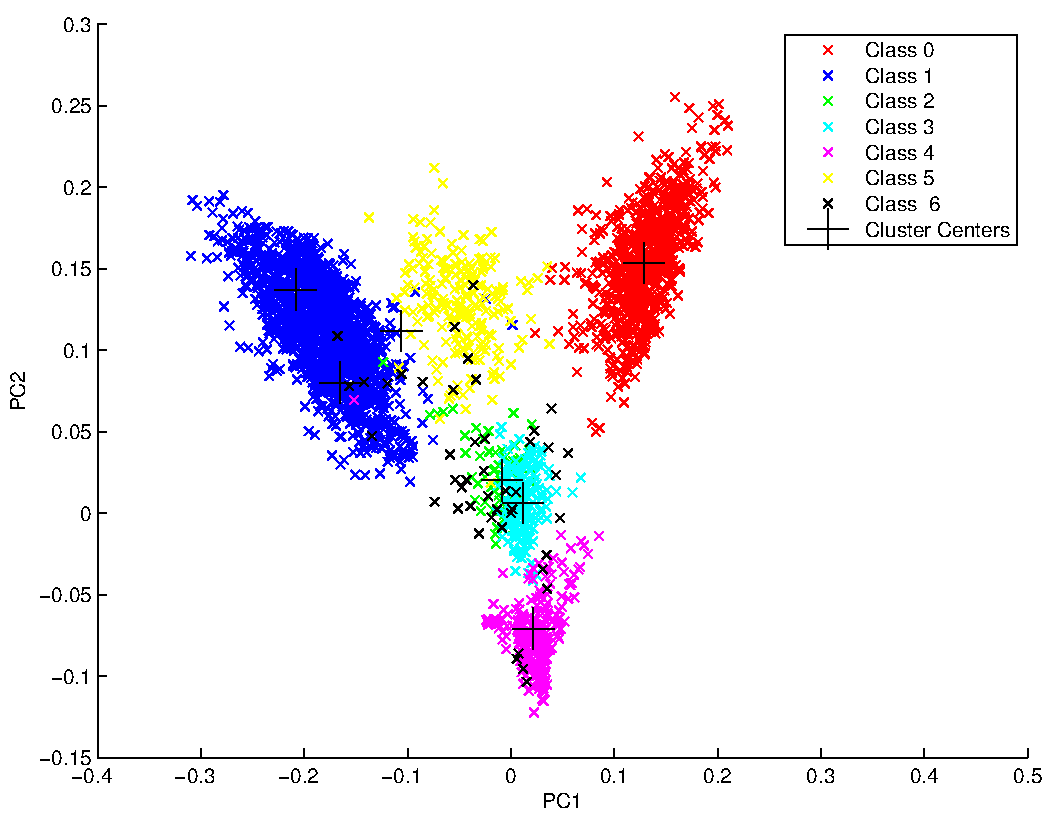
\includegraphics[width=.5\textwidth]{7meansclusters.pdf}}
  \subfloat[\hfill]{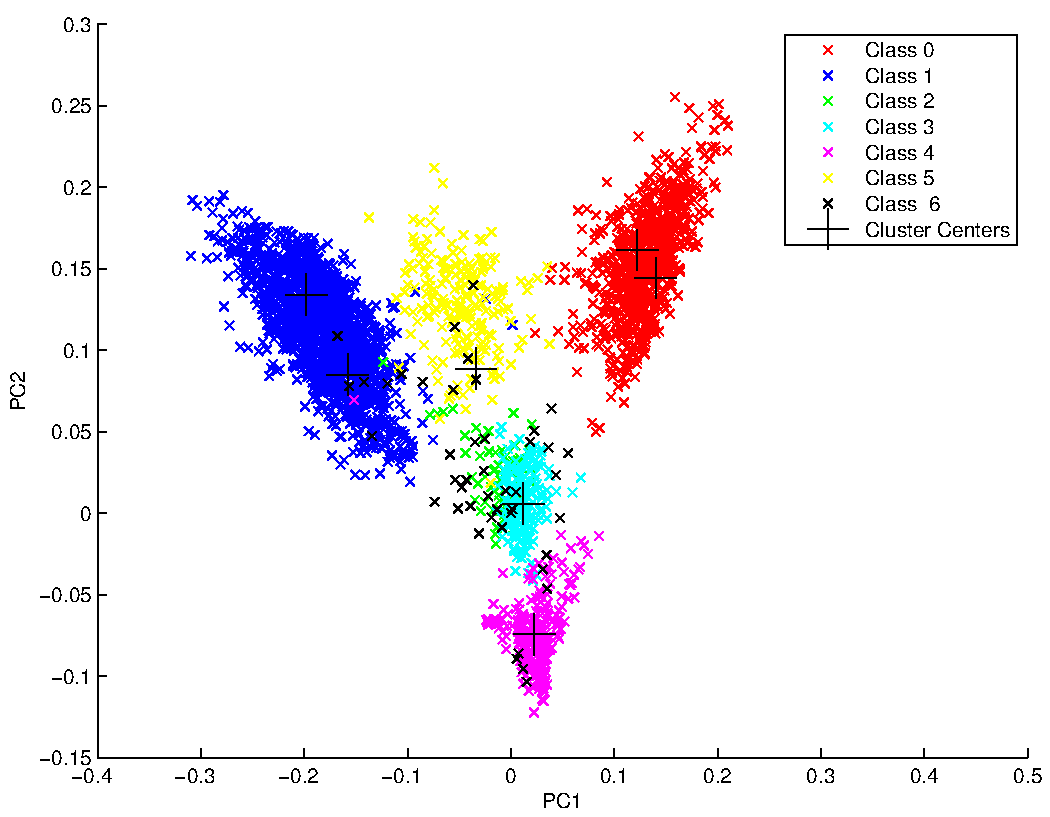
\includegraphics[width=.5\textwidth]{7meansclusters2.pdf}}
  \caption{Cluster centers projected into the training data for different results of kmeans}
  \label{fig:7meansclusters}
\end{figure}

\section{Question 4}
\begin{enumerate}
\item Traditional overfitting: I think it is safe to say that for the methods we want to apply, our training data set is large enough. Since we only ever use algorithms with two hyperparameters, this is likely not a source of overfitting. Because of the fact that all algorithms we tried also performed reasonably well on the test data set, we can relatively safely say that we do not have an overfitting problem anywhere. However, it would of course be possible to use very complex predictors to get overfitting even on our training set, for example by using a very large neural network or a high-order polynomial. There might also be a problem because there are significantly fewer data patterns for higher classes than lower ones, which means these could in fact become too few for reasonable training relatively fast. Additionally, the error class, since patterns in it can be anything but a valid value for the other classes, is relatively hard to describe, which is why an algorithm trained to detect values for this class will likely overfit.
\item Parameter tweak overfitting: This is, of course, always possible, no matter which data set or application is used. We used cross-validation to find the best hyperparameters whereever possible and never used the test set for any training purposes whatsoever, so we probably do not have a big problem in this regard. The differences in the frequency of different classes in both sets, however, might tempt us to choose parameters which perform well on overrepresented classes and badly on underrepresented classes. This is at least partly the case, as the error class, which only includes a small part of the training set, is classified quite badly by most algorithms that we use.
\item Brittle measure: The explanation names leave-one-out cross-validation, which we have used, as a brittle measure. But we only used it for choosing good hyperparameters, the actual evaluation of the results always relied solely on the performance on the test set. Yet there are some problems with our data, for example the fact that the data patterns are ordered by class, which might for example be a problem for cross-validation if the groups are chosen badly. 
\item Bad statistics: Since we do not make any confidence statements throughout the exam, we should be safe here. Otherwise we would have to make sure we do not treat our cross-validation data as iid. In this case we should also think of the sampling bias that may exist in the data, as suggested in Question 6.
\item Choice of measure: It would be possible to make our results look better by choosing different performance measures, since there will always be a performance measure that yields a better result on a specific data set than a different one would. Throughout the exam, we always used the error percentage, which sounds like a reasonable thing to do and makes the different algorithms comparable. It is also an absolute measure, which in my opinion is a lot safer to use than any kind of relative measures. But it is true that this choice might hide some details, for example a very bad performance of an algorithm on a specific class which is underrepresented in the data set (which is the case in our data sets).
\item Incomplete Prediction: Question 6 illustrates one step of many which would be necessary to replace a multi-class decision by a series of binary decisions, so this would obviously be possible with our data. However, in all other cases, we have used real multi-class predictors. For our data set, one might argue that it could be a good idea to remove the error class from the multi-class classification, since it is not actually a class of points with a set of common attributes, and determine if there is an error before the multi-class classification or afterwards, for example for low confidence levels. In a way, one might say that using multi-class prediction on our data set including the error class illegaly mixes a multi-class and a binary decision.
\item Human-loop overfitting: There are some points where humans were involved in creating the data set (assignment to categories) or human decisions are involved in the algorithm (initialization of kmeans). We can only guess that the assignment has been done correctly and without distorting the data in any way (i.e. by categorizing groups as errors when they are not clearly visible). We used random initialization for kmeans, but there is of course a human factor present in selecting a result after running it multiple times. Human interaction is obviously present during model selection, but this is by design.
\item Data set selection: It is claimed that the data set is the result of an algorithm scanning video footage. There is no way for us to know is there was some kind of preselection of a specific part of the data, which is definitely possible. If not, the data set might still be influenced in some way by the other algorithm, which might, for example, only detect ROIs which are very clearly identifyable, which would make the work for our algorithm a lot easier. The fact that the data source is somewhat natural can give us some confidence, but we cannot rule anything out here.
\item Reprobleming: There does not seem to be a problem of this kind in our case, since our data set does not allow any predictions other than the ones we made and we never took a step back from our initial goal. The step towards a binary decision in question 6 might be regarded as reprobleming, however.
\item Old datasets: Since we have never seen this data set and Christian said it contains footage of his two favorite teams, we can assume that he made it and made it specifically for this assignment, which means this is not a problem.
\end{enumerate}

\section{Question 5}

I chose Linear Discriminant Analysis for the linear classifier and $k$-Nearest Neighbour for the non-linear one. Both are rather basic algorithms which do not rely too much in finding the right hyperparameters, so that the results can be compared easily. I implemented both algorithms myself by extending my group's implementations for the mandatory assignments. The implementations can be found in \texttt{q5knn.m} and \texttt{q5lda.m} and referenced files, respectively. 

I performed a grid search using 5-fold cross-validation on the test set to find the optimal value of $k$ and used the found value throughout the exercise. In $k$-NN, ties are broken at random. The results of the grid search can be found in table ~\ref{tab:knncv}. Based on this we can now choose $k=1$ for the rest of the exercise, as it gave us the lowest cross-validation error percentage.

\begin{table}[h!]
  \centering
  \begin{tabular}{l|c|c|c|c|c|c|c|c}
    \backslashbox{Dataset}{$k$} & 1 & 2 & 3 & 5 & 7 & 9 & 20 & 50 \\
    \hline
    \texttt{trainInput} & 0.7373 & 0.8044 & 0.7709 & 0.8043 & 0.9382 & 0.9047 & 1.2398 & 1.8096 \\
  \end{tabular}
  \caption{Cross-validation error of $k$-NN on the train set for different values of $k$ in percent}
  \label{tab:knncv}
\end{table}

LDA produced an error of $0.37\%$ on the training and $7.44\%$ on the test data. $k$-NN produced an error of 5.917\% on the test set. For $k=1$, the error on the training set is, of course, 0. If we choose the second best option, $k=3$, the error on the training set is 0.503\%. LDA therefore performs slightly better on the training set, whereas $k$-NN is slightly better on the test set. Both algorithms have worse results on the test set, which is to be expected, but they still perform well enough to give reasonable classifications. The grid search for $k$-NN also seems to have provided us with a good result, which is demonstrated by $k$-NN's results with other values of $k$ (table ~\ref{tab:knnerror}).

\begin{table}[h!]
  \centering
  \begin{tabular}{l|c|c|c|c|c|c|c|c}
    \backslashbox{Dataset}{$k$} & 1 & 2 & 3 & 5 & 7 & 9 & 20 & 50 \\
    \hline
    \texttt{trainInput} & 0.00 & 0.4357 & 0.5027 & 0.6367 & 0.7373 & 0.8378 & 1.1394 & 1.6421 \\
    \texttt{testInput} & 5.9168 & 6.1511  & 5.9168 & 6.0340 & 6.6198 & 6.6784 & 6.9127 & 7.0885 \\
  \end{tabular}
  \caption{Error of $k$-NN for different values of $k$ in percent}
  \label{tab:knnerror}
\end{table}

If we plot the results of LDA on the test set (fig. ~\ref{fig:ldaplot}), again reduced to the first two principal components, we see that the results indeed look reasonable. There seems to be a block of points assigned to the error class which probably does not belong there. This is not surprising, since LDA always finds a mean for each class and points close to this mean will very likely be assigned to the respective class. This can, and in this case does, lead to bad results if one class (the error class) is spread out a lot and overlaps with other classes. 

\begin{figure}
  \centering
  \subfloat[\hfill]{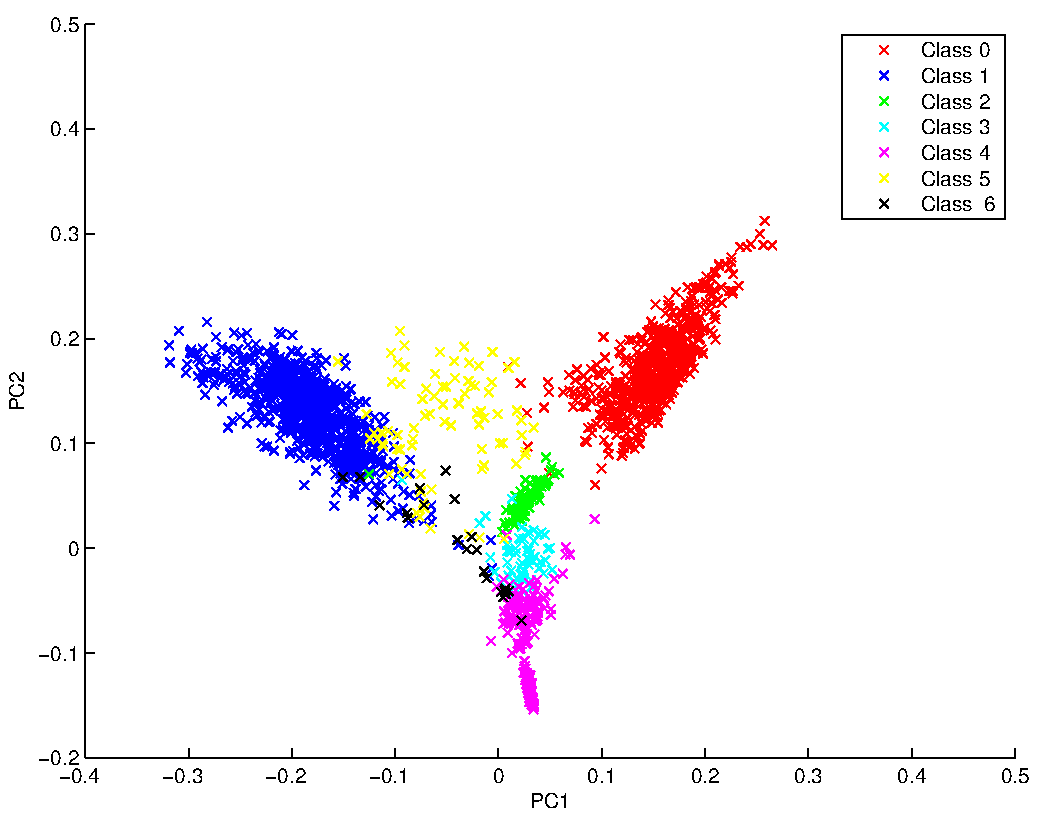
\includegraphics[width=.6\textwidth]{ldaplot.pdf}}
  \caption{Classification result of LDA on the test set}
  \label{fig:ldaplot}
\end{figure}

\section{Question 6}
I implemented the computation for $\sigma_{Jaakkola}$ in \texttt{jaakkola.m}. For the training data, it computes $\sigma_{Jaakkola} = 0.2592$, which gives us $\gamma_{Jaakkola} = 7.4397$. I chose $b=2$. 

For the implementation of the SVM, I used LIBSVM via its Matlab interface, since it is the standard tool for using SVMs and I've already worked with it in the madatory assignments. I built wrappers for LIBSVM's \texttt{svmtrain} and \texttt{svmpredict} functions and one which calls LIBSVM's integrated cross-validation function. All functions are called with default parameters, i.e. a C-SVM with a Gaussian kernel as specified in the question. For details, see \texttt{q6.m} and referenced files.

As I stated, I performed the grid search using $5$-fold cross-validation with LIBSVM's builtin cross-validation function. The results can be seen in table ~\ref{tab:crossval}. There are several parameter configurations with the same high accuracy. I chose the one with the lowest value for $C$, since a higher value for $C$ gets us closer to a hard-margin SVM, which is more likely to have overfitting. The best parameter configuration for the training data is therefore $C=1$ and $\gamma=59.517771$ (which is $\gamma=\gamma_{Jaakkola}*b^3$).

\begin{table}[h!]
  \centering
  \begin{tabular}{l|c|c|c|c|c|c|c|c}
    $\gamma$ & 0.929965 & 1.859930 & 3.719861 & 7.439721 & 14.879443 & 29.758885 & 59.517771 \\
    \backslashbox{$C$}{$i$} & -3 & -2 & -1 & 0 & 1 & 2 & 3 \\
    \hline
    0.5 & 84.5118 & 93.9394 & 97.3064 & 97.6431 & 97.6431 & 98.9899 & 99.3266 \\
    1 & 93.9394 & 97.3064 & 97.6431 & 97.6431 & 98.6532 & 99.3266 & 99.6633 \\
    2 & 97.3064 & 97.6431  & 97.6431 & 98.3165 & 99.3266 & 99.6633 & 99.3266 \\
    4 & 97.6431 & 97.6431 & 98.3165 & 99.6633 & 99.6633 & 99.3266 & 99.3266 \\
    8 & 97.6431 & 98.3165 & 98.9899 & 99.6633 & 99.3266 & 99.3266 & 99.3266 \\
  \end{tabular}
  \caption{Error of SVM classification for different parameter configurations}
  \label{tab:crossval}
\end{table}

Training the SVM on the entire training data set and classifying with the resulting model gives us $99.6633\%$ accuracy on the training data and $99.1342\%$ on the test data. Both are very good results which surpass LDA and $k$-NN by some margin. The added complexity of the SVM seems to help a lot to capture the features of the underlying distribution, so that even the hard-to-detect error class and the partly-overlapping classes 2 and 3 can be distinguished very well. Additionally, there seems to be almost no overfitting whatsoever, as the performance on the test set is very close to the one on the training set. 

\section{Question 7}

First part:

From the lecture slides we know the discrimation function
\begin{eqnarray}
\delta_k (x) &= x^T \Sigma^{-1} \mu_k - \frac{1}{2} \mu_k^T \Sigma^{-1} \mu_k + ln(l_k /l)
\end{eqnarray}
LDA classification assigns a pattern $x$ to a class $y$ according to
\begin{eqnarray}
y&=argmax_k \delta_k(x)
\end{eqnarray}
In binary classification, this means class 2 is chosen over class 1 if 
\begin{eqnarray}
\delta_2 (x) &> \delta_1 (x)
\end{eqnarray}
If we expand this, we get
\begin{eqnarray}
x^T \Sigma^{-1} \mu_2 - \frac{1}{2} \mu_2^T \Sigma^{-1} \mu_2 + ln(l_2 /l) &> x^T \Sigma^{-1} \mu_1 - \frac{1}{2} \mu_1^T \Sigma^{-1} \mu_1 + ln(l_1 /l) 
\end{eqnarray}
which can be reordered to give us the equation we want:
\begin{eqnarray}
x^T \Sigma^{-1} (\mu_2 - \mu_1) &> frac{1}{2}\mu_2^T \Sigma^{-1} \mu_2 - \frac{1}{2}\mu_1^T\Sigma^{-1}\mu_1 + ln \frac{l_1}{l} - ln \frac{l_2}{l}
\end{eqnarray}

Second part:

For the second part, we follow the steps of Bishop 4.1.5. Since we want to minimize the error, we want to set its partial derivatives
\begin{eqnarray}
E=\sum\limits_{i=1}^l \frac{1}{2}(y_i - \beta_0 -\beta^Tx_i )^2 \\
\frac{\partial E}{\partial \beta_0}= \sum\limits_{i=1}^l (y_i - \beta_0 - \beta^Tx_i)\\
\frac{\partial E}{\partial \beta^T}= \sum\limits_{i=1}^l (y_i - \beta_0 - \beta^Tx_i)x_i
\end{eqnarray}
to zero. We assume that the elements $x_i$ are ordered so that $x_1..x_{l_1}$ belong to class 1 and the rest belongs to class 2. For (7), this gives us 
\begin{align*}
0&=\sum\limits_{i=1}^l(y_i-\beta_0-\beta^Tx_i) \\
0&=\sum\limits_{i=1}^{l_1} (-\frac{l}{l_2} -\beta_0-\beta^Tx_i) + \sum\limits_{i=l_1+1}^{l_2} (\frac{l}{l_2}-\beta_0-\beta^Tx_i) 
\end{align*}
Because of 
\begin{align*}
\mu&=\frac{1}{l} \sum\limits_{i=1}^{l}x_i
\end{align*}
this gives us
\begin{align*}
0&=l_2 \frac{l}{l_2}-l_1 \frac{l}{l_1}-l\beta_0-l\beta^T\mu \\
\beta_0 &= -\beta^T\mu
\end{align*}
We now set (8) to zero
\begin{align*}
0&=\sum\limits_{i=1}^{l} (y_i - \beta_0 -\beta^Tx_i)x_i \\
&=\sum\limits_{i=}^{l_1} - \frac{l}{l_1}x_i + \sum\limits_{i=l_1+1}^{l_2} \frac{l}{l_2}x_i - \sum\limits_{i=1}^l \beta_0x_i - \sum\limits_{i=1}^l (\beta^Tx_i)x_i \\
&=-l\mu_1 +l\mu_2 -l\beta_0\mu-\sum\limits_{i=1}^l(\beta^Tx_i)x_i
\end{align*}
We use $\beta_0=-\beta^T\mu$ to get
\begin{align*}
l(\mu_1-\mu_2) &= l(\beta^T\mu)\mu-(\sum\limits_{i=1}^l x_ix_i^T)\beta \\
&=(l\mu\mu^T-\sum\limits_{i=1}^l x_ix_i^T)\beta \\
&=(-\sum\limits_{i=1}^l (x_i-\mu)(x_i-\mu)^T)\beta \\
&=(-\sum\limits_{i=1}^{l_1}(x_i-\mu)(x_i-\mu)^T) - \sum\limits_{i=l_1+1}^{l_2}(x_i-\mu)(x_i-\mu)^T)\beta 
\end{align*}
We now calculate 
\begin{align*}
\sum\limits_{i=1}^{l_1}(x_i-\mu)(x_i-\mu)^T &= \sum\limits_{i=1}^{l_1} [(x_i-\mu)+(\mu-\mu_1)][(x_i-\mu)+(\mu-\mu_1)]^T \\
&=\sum\limits_{i=1}^{l_1} (x_i-\mu)(x_i-\mu)^T + \sum\limits_{i=1}^{l_1} (x_i-\mu)(\mu-\mu_1)^T + \sum\limits_{i=1}^{l_1} (\mu-\mu_1)(x_i-\mu)^T + \sum\limits_{i=1}^{l_1} (\mu-\mu_1)(\mu-\mu_1)^T \\
&=\sum\limits_{i=1}^{l_1} (x_i-\mu)(x_i-\mu)^T + \sum\limits_{i=1}^{l_1} (\mu-\mu_1)(\mu-\mu_1)^T +2(\sum\limits_{i=1}^{l_1} x_i\mu^T - \sum\limits_{i=1}^{l_1} x_i\mu_1^T - \sum\limits_{i=1}^{l_1} \mu\mu_1^T + \sum\limits_{i=1}^{l_1} \mu\mu_1^T) \\
&=\sum\limits_{i=1}^{l_1} (x_i-\mu)(x_i-\mu) + l_1\mu\mu^T -l_1\mu\mu^T -l_1\mu_1\mu^T + l_1\mu_1\mu_1^T +2(l_1\mu_1\mu^T - l_1\mu_1\mu_1^T - l_1\mu\mu_1^T + l_1\mu\mu_1^T)\\
&=\sum\limits_{i=1}^{l_1}(x_i-\mu)(x_i-\mu)^T - l_1(\mu-\mu_1)(\mu-\mu_1)^T
\end{align*}
When we do the same for class two and substitute, we get
\begin{align*}
l(\mu_2 - \mu_1) &= [- \sum\limits_{i=1}^{l_1} (x_i-\mu_1)(x_i-\mu_1)^T - \sum\limits_{i=l_1+1}^{l_2} (x_i-\mu_2)(x_i-\mu_2)^T -l_1(\mu-\mu_1)(\mu-\mu_1)^T -l_2(\mu-\mu_2)(\mu-\mu_2)^T]\beta
\end{align*}
Using Bishop (4.36), we get 
\begin{align*}
-l_1(\mu-\mu_1)(\mu-\mu_1)^T - l_2(\mu-\mu_2)(\mu-\mu_2)^T &= -\frac{l_1l_2}{l}\Sigma_B
\end{align*}
where $\Sigma_B$ is the between-class covariance matrix (Bishop 4.27). We now use this and write the within-class covariance matrix as $\Sigma$ (Bishop 4.28), so we get
\begin{align*}
l(\mu_2-\mu_1)=[\Sigma+\frac{l_1l_2}{l} \Sigma_B]\beta
\end{align*}
from which we can conclude that $\beta$ is always in the direction
\begin{align*}
\beta \propto \Sigma^{-1}(\mu_2-\mu_1)
\end{align*}

\section{Question 8}
Using scalar target values for multi-class classification with regression is a bad idea. The size and order of the class labels, which (usually) should not influence the performance of the algorithm at all, would have a huge impact on the classification. Using ${0,1,..,6}$ as the targets, as suggested in the question, would mean that classes 3 and 4 are somehow more similar to each other than classes 1 and 6. If this assumption is not supported by our data, which for our example it is not, this assumption can lead to absurd results. For example, if the algorithm is not sure if a given point belongs to class 2 or 4, it might output a value between those labels, which would mean it is put in class 3, which for our data does not make sense at all.

This is the reason why other means, for example indicator matrices (in our case \{$(1, 0, 0, 0, 0, 0, 0)^T$  ...  $(0, 0, 0, 0, 0, 0, 1)^T$\}) should be used as targets instead.

\end{document}
